\documentclass[a4paper,12pt]{report}
\usepackage[utf8]{inputenc}
\usepackage[T1]{fontenc}
\usepackage{lmodern}
\usepackage{mathtools}
\usepackage[catalan]{babel}
\usepackage{hyperref}
\usepackage{graphicx}
\usepackage{acronym}
\usepackage{eurosym}
\usepackage{pgfplots}
\usepackage[backend=biber]{biblatex}
\usepackage[auth-sc]{authblk}

\addbibresource{biblio/main.bib}

\date{}
\begin{document}

\acrodef{ia}[IA]{{inteligència artificial}}
\acrodef{ann}[ANN]{{xarxa neuronal artificial}}


\title{
	{\bf Filosofia del Software i Intel·ligència Artificial} \\
	Procediments
}
\author{
	Oriol Ventosa \and
	Marc Ferré \and
	Gonzalo Palacios \and
	Pol Gómez
}

\maketitle

\tableofcontents

\chapter{Introducció}
Els procediments del projecte de recerca es basen en la realització de diferents \emph{demos} (demostracions)
que tenen la intenció de oferir una introducció a les aplicacions de la \ac{ia}.

S'ha utilitzat el llenguatge de programació C++, i les llibreríes SFML \autocite{sfmllib} (per a gràfics) i FANN \cite{fannlib} (per a la
creació i entrenament de xarxes neuronals).

Les demos (junt amb el seu estat de progrés actual) són les següents:

\begin{itemize}
\item \emph{Demo 1} - joc de futbol sala (5 jugadors per equip), aprenentatje 'per esforç' (reinforcement) amb \ac{ann} evolutiva, estat inicial
\item \emph{Demo 2} - reconeixement de caràcters 0-9, \ac{ann}, estat avançat (ajustament de paràmetres d'aprenentatge, etc)
\item \emph{Demo 3} - conducció automàtica (circuit simple), reinforcement amb \ac{ann} evolutiva, estat inicial (físiques de conducció)
\item \emph{Demo 4} - ?
\end{itemize}

\emph{* La llista de demostracions pot variar fins a la versió final *}


\chapter{Xarxes Neuronals Artificials}
Les \emph{xarxes neuronals artificials} (ANN) són \emph{models computacionals 
inspirats pel sistema nerviós central dels animals (en particular, el cervell)} \autocite{nnpatrec}.

L'estructura d'una \ac{ann} és semblant a la d'un circuit electrònic: hi ha una capa o \emph{layer}
de $ q $ neurones d'entrada, o \emph{inputs}, i un layer de $ p $ neurones de sortida, o \emph{outputs}.
Això permet representar la seva estructura com si fos una funció matemàtica, $ f(x_0, x_1, ..., x_q) = \{y_0, y_1, ..., y_p\} $,
és a dir: un conjunt $ x $ d'entrades formen un conjunt $ y $ de sortides \ref{simple_ann}.

\begin{figure}[ht!]
\centering
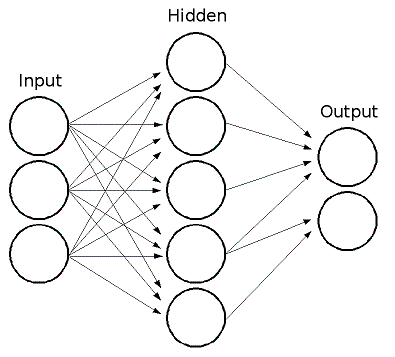
\includegraphics[width=80mm]{data/nn_simple.png}
\caption{El propòsit del layer \emph{hidden} s'explicarà més endavant.}
\label{simple_ann}
\end{figure}

La tasca principal d'una xarxa neuronal \emph{supervisada} és realitzar una \emph{aproximació de funció},
és a dir, a partir d'un seguit de valors de la funció (anomenat \emph{training set}), $ f(a) = b $, crear un model que s'ajusti a les dades
que se li ha subministrat \ref{func_approx}. Podríem, per exemple, entrenar una \ac{ann} per a que realitzés
una aproximació de la funció $ sin(x)$, però és més interessant entrenar-la amb objectius més sofisticats; tot
problema determinista que es pugui reduir a \emph{produir unes sortides a partir d'uns valors d'entrada}, es pot
solucionar, molt probablement, amb una xarxa neuronal.

\begin{itemize}
\item \emph{Conduir un cotxe:} la posició, la velocitat, els cotxes adjacents, la carretera... una gran quantitat d'entrades. La nova direcció, 
accelerar o frenar, com a sortides.
\item \emph{Predir el flux del mercat de valors:} la pendent de la gràfica del valor d'una acció, els últims moviments, els últims compradors...
la xarxa s'ha entrenat amb dades històriques, i l'historia es repeteix. El moviment de l'accionista com a sortida.
\item \emph{Reconèixer caràcters:} aquesta és la nostra parada per a continuar amb l'explicació de les \ac{ann}. El conjunt de píxels que formen 
l'imatge d'un caràcter com a entrades, i el número que representen els píxels com a sortida. És un exemple fàcil d'aplicar i enriquidor.
\end{itemize}

\begin{figure}[ht!]
\centering
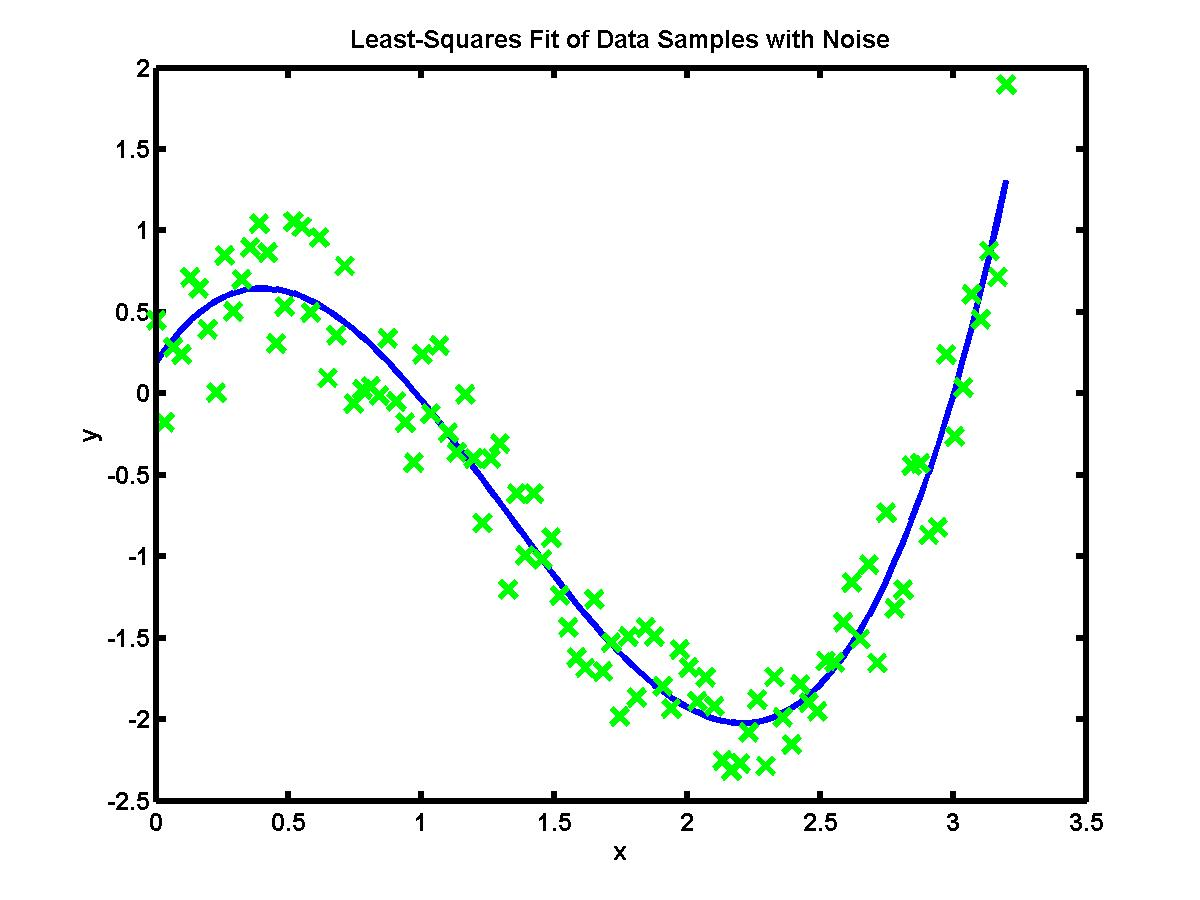
\includegraphics[width=80mm]{data/func_approx.jpg}
\caption{Exemple d'aproximació de funció. Els punts verds són els valors subministrats, el training set,
i la línia blava la funció que s'ha aproximat.}
\label{func_approx}
\end{figure}

\chapter{Futbol Sala Intel·ligent}
La demostració 1


\chapter{Reconeixement de Caràcters}
\begin{figure}[ht!]
\centering
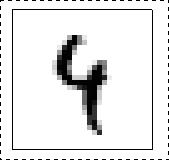
\includegraphics[width=35mm]{data/confusing_2.png}
\caption{4 o 9? La nostra \ac{ann} creu amb un 100\% de certesa que és un 4, i amb un 47\% de certesa que és un 9.}
\label{certesa}
\end{figure}

Podem visualitzar perfectament el model neuronal que representa un problema de reconeixement de caràcters: la nostra
base de dades, o \emph{dataset}, consisteix de 1000 formes d'escriure cada número, del 0 al 9. És a dir, la xarxa neuronal
no aprendrà només com en Xavi dibuixa el 5, sinó que aprendrà també com el dibuixen 999 persones diferents, exposició suficient per
a poder realitzar una extracció de característiques, o \emph{feature extraction}.

Això és vital, extreure característiques, i per aconseguir-ho necessitem utilitzar un layer addicional, el \emph{hidden}. 
Si realitzéssim l'entrenament amb un layer d'inputs i un layer d'outputs, la interpolació que es produiria seria lineal,
es a dir, es realitzaria un motlle amb el qual es compararia qualsevol imatge, i la major part d'elles no entrarien dins
els paràmetres del motlle (la \emph{dimensionalitat} és única). El que volem es que la xarxa neuronal descobreixi que el número
vuit hauria de tenir dos cercles, que el set és com un 1, però amb un vèrtex desplaçat, que el quatre pot ser un triangle o un
quadrat obert per amunt, ... imagines haver de programar totes aquestes condicions de forma manual? Si no t'ho pots imaginar, 
et deixem la resposta: és un suïcidi.

La xarxa neuronal utilitza el layer hidden per a fabricar un \emph{motlle flexible} i sofisticat, que reconeix certes característiques
en comptes de forçar un model universal. Aquí és quan les \ac{ann}s brillen per complet; són capaces de crear una \emph{caixa negra}
extremadament interconnectada i intel·ligent, que sembla utilitzar raonament, evidentment, intel·ligent. En realitat no hi ha màgia, 
és tot producte d'un magnífic i complex model matemàtic.

\begin{figure}[ht!]
\centering
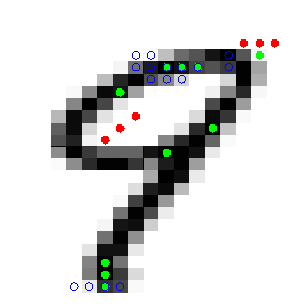
\includegraphics[width=45mm]{data/extraction-0.png}
\caption{Exemple d'extracció de característiques. Gràcies a \href{http://clopinet.com/isabelle/Projects/ETH/}{Isabelle Guyon} \autocite{guyonfe}.}
\label{extracció}
\end{figure}

Nosaltres hem extret un dataset \href{http://cis.jhu.edu/~sachin/digit/digit.html}{derivat} del majestuós \href{http://yann.lecun.com/exdb/mnist/}{MINST} (derivat al seu torn del NIST)
que ofereix deu arxius binaris amb 28x28 píxels per imatge, 1 byte per píxel. El procés que hem seguit per a produir una demostració efectiva de les 
xarxes neuronals en reconeixement de caràcters ha estat el següent:

\begin{enumerate}
\item Establint un índex d'arxiu (del 0 al 9) i un índex d'imatge (del 0 al 999), carreguem l'arxiu adient a l'índex i l'emmagatzemem en un gran vector. A través del teclat, podem
navegar les diferents imatges de cada nombre. Es carrega llavors l'imatge en un panell, per a poder-ho visualitzar.
\item Prement la tecla \emph{C} (de \emph{convert}), el programa crea un arxiu adequat al format que utilitza la llibreria de \ac{ann}s. Importa i normalitza una certa quantitat 
de mostres en un sol arxiu, perfecte per a entrenar la \ac{ann}.
\item Prement la tecla \emph{L} (de \emph{learn}, aprendre), el programa crea una \ac{ann} amb 784 neurones d'entrada, 392 neurones hidden, i 10 neurones de sortida: 3 milions de connexions. Utilitza la 
llibreria per a llegir l'arxiu convertit anteriorment, i entrena la \ac{ann} amb un mètode popular anomenat \emph{backpropagation}. Consisteix en establir uns pesos aleatoris 
en totes les neurones, a l'inici del programa. Llavors, donat un set d'entrenament, prova a calcular el resultat de la xarxa amb unes certes entrades del set, i el compara amb el resultat
que hauria d'obtindre. A través de l'error obtingut, realitza una marxa enredera recursiva, i ajusta els pesos de les neurones de forma que produeixin outputs similars a la que
estableix el set d'entrenament. Realitza tot aquest procés per cada imatge de les 7500 que li deixem per a entrenar.
\item Prement la tecla \emph{T} (de \emph{test}, comprovar), el programa utilitza l'índex corresponent a l'imatge que l'usuari està veient en pantalla, i estableix els seus píxels
com a entrades d'una \ac{ann} creada a partir de l'entrenament anterior. Produeix llavors, la desitjada sortida que estàvem esperant, imprimint a la consola (l'objectiu és dibuixar un gràfic)
la certesa per cada número de l'1 al 9.
\end{enumerate}


\begin{figure}[ht!]
\centering
\includegraphics[width=65mm]{data/test.png}
\caption{Sortida de la nostra xarxa neuronal, per a un estrany número 8. En molts casos, els números 5, 6 i 8 comparteixen característiques. La xarxa neuronal les descobreix.}
\label{output}
\end{figure}



\printbibliography

\end{document}
